\begin{figure}
\centering
\textbf{Podcast transcripts}
\begin{minipage}{0.25\textwidth}
\vspace*{2mm}
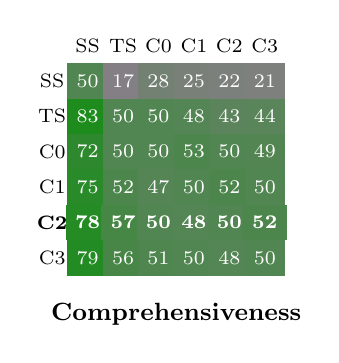
\begin{tikzpicture}[scale=0.45]
  \def\rowlabels{{"SS","TS","C0","C1","C2","C3"}}
  \def\collabels{{"SS","TS","C0","C1","C2","C3"}}
  \foreach \y [count=\n] in {
      {50, 17, 28, 25, 22, 21},
      {83, 50, 50, 48, 43, 44},
      {72, 50, 50, 53, 50, 49},
      {75, 52, 47, 50, 52, 50},
      {78, 57, 50, 48, 50, 52},
      {79, 56, 51, 50, 48, 50},
    } {

      % heatmap tiles
      \foreach \x [count=\m] in \y {
      \pgfmathsetmacro{\z}{(\x-20)*(100/60)}
        \ifnum\n=5
            \node[fill=ForestGreen!\z!gray, minimum size=4.5mm, text=white, font=\scriptsize] at (\m,-\n) {\textbf{\x}};
        \else
            \node[fill=ForestGreen!\z!gray, minimum size=4.5mm, text=white, font=\scriptsize] at (\m,-\n) {\x};
        \fi
      }
    }

  % row labels
  \foreach \a [count=\i] in {0,...,5} {
    \ifnum\a=4
        \node[minimum size=4.5mm, font=\scriptsize] at (0,-\i) {\textbf{\pgfmathparse{\rowlabels[\a]}\pgfmathresult}};
    \else
        \node[minimum size=4.5mm, font=\scriptsize] at (0,-\i) {\pgfmathparse{\rowlabels[\a]}\pgfmathresult};
    \fi
    }
  % column labels
  \foreach \a [count=\i] in {0,...,5} {
    \node[minimum size=4.5mm, font=\scriptsize] at (\i,0) {\pgfmathparse{\collabels[\a]}\pgfmathresult};
  }
  \node[below, align=center, font=\small] at (3.5, -7) {\textbf{Comprehensiveness}};
\end{tikzpicture}
\vspace*{2mm}
\end{minipage}%
\begin{minipage}{0.25\textwidth}
\vspace*{2mm}
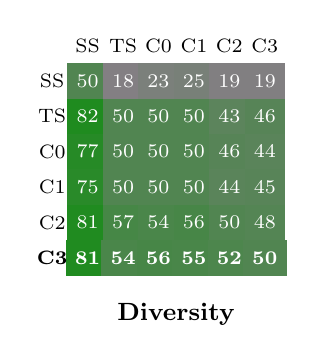
\begin{tikzpicture}[scale=0.45]
  \def\rowlabels{{"SS","TS","C0","C1","C2","C3"}}
  \def\collabels{{"SS","TS","C0","C1","C2","C3"}}
  \foreach \y [count=\n] in {
     {50, 18, 23, 25, 19, 19},
     {82, 50, 50, 50, 43, 46},
     {77, 50, 50, 50, 46, 44},
     {75, 50, 50, 50, 44, 45},
     {81, 57, 54, 56, 50, 48},
     {81, 54, 56, 55, 52, 50},
    } {

      % heatmap tiles
      \foreach \x [count=\m] in \y {
      \pgfmathsetmacro{\z}{(\x-20)*(100/60)}
        \ifnum\n=6
            \node[fill=ForestGreen!\z!gray, minimum size=4.5mm, text=white, font=\scriptsize] at (\m,-\n) {\textbf{\x}};
        \else
            \node[fill=ForestGreen!\z!gray, minimum size=4.5mm, text=white, font=\scriptsize] at (\m,-\n) {\x};
        \fi
      }
    }

  % row labels
  \foreach \a [count=\i] in {0,...,5} {
    \ifnum\a=5
        \node[minimum size=4.5mm, font=\scriptsize] at (0,-\i) {\textbf{\pgfmathparse{\rowlabels[\a]}\pgfmathresult}};
    \else
        \node[minimum size=4.5mm, font=\scriptsize] at (0,-\i) {\pgfmathparse{\rowlabels[\a]}\pgfmathresult};
    \fi
    }
  % column labels
  \foreach \a [count=\i] in {0,...,5} {
    \node[minimum size=4.5mm, font=\scriptsize] at (\i,0) {\pgfmathparse{\collabels[\a]}\pgfmathresult};
  }
  \node[below, align=center, font=\small] at (3.5, -7) {\textbf{Diversity}};
\end{tikzpicture}
\vspace*{2mm}
\end{minipage}%
\begin{minipage}{0.25\textwidth}
\vspace*{2mm}
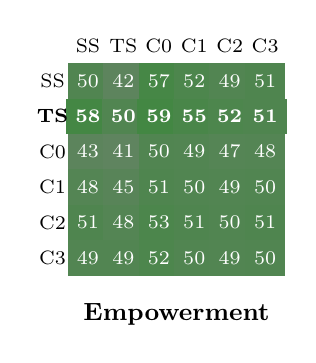
\begin{tikzpicture}[scale=0.45]
  \def\rowlabels{{"SS","TS","C0","C1","C2","C3"}}
  \def\collabels{{"SS","TS","C0","C1","C2","C3"}}
  \foreach \y [count=\n] in {
    {50, 42, 57, 52, 49, 51},
    {58, 50, 59, 55, 52, 51},
    {43, 41, 50, 49, 47, 48},
    {48, 45, 51, 50, 49, 50},
    {51, 48, 53, 51, 50, 51},
    {49, 49, 52, 50, 49, 50},
    } {

      % heatmap tiles
      \foreach \x [count=\m] in \y {
        \pgfmathsetmacro{\z}{(\x-20)*(100/60)}
        \ifnum\n=2
            \node[fill=ForestGreen!\z!gray, minimum size=4.5mm, text=white, font=\scriptsize] at (\m,-\n) {\textbf{\x}};
        \else
            \node[fill=ForestGreen!\z!gray, minimum size=4.5mm, text=white, font=\scriptsize] at (\m,-\n) {\x};
        \fi
      }
    }

  % row labels
  \foreach \a [count=\i] in {0,...,5} {
    \ifnum\a=1
        \node[minimum size=4.5mm, font=\scriptsize] at (0,-\i) {\textbf{\pgfmathparse{\rowlabels[\a]}\pgfmathresult}};
    \else
        \node[minimum size=4.5mm, font=\scriptsize] at (0,-\i) {\pgfmathparse{\rowlabels[\a]}\pgfmathresult};
    \fi
    }
  % column labels
  \foreach \a [count=\i] in {0,...,5} {
    \node[minimum size=4.5mm, font=\scriptsize] at (\i,0) {\pgfmathparse{\collabels[\a]}\pgfmathresult};
  }
  \node[below, align=center, font=\small] at (3.5, -7) {\textbf{Empowerment}};
\end{tikzpicture}
\vspace*{2mm}
\end{minipage}%
\begin{minipage}{0.25\textwidth}
\vspace*{2mm}
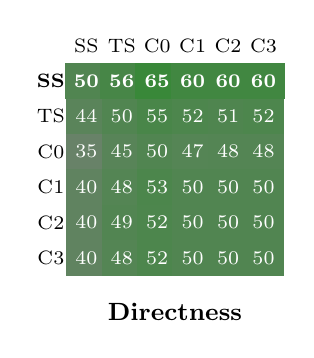
\begin{tikzpicture}[scale=0.45]
  \def\rowlabels{{"SS","TS","C0","C1","C2","C3"}}
  \def\collabels{{"SS","TS","C0","C1","C2","C3"}}
  \foreach \y [count=\n] in {
      {50, 56, 65, 60, 60, 60},
      {44, 50, 55, 52, 51, 52},
      {35, 45, 50, 47, 48, 48},
      {40, 48, 53, 50, 50, 50},
      {40, 49, 52, 50, 50, 50},
      {40, 48, 52, 50, 50, 50},
    } {

      % heatmap tiles
      \foreach \x [count=\m] in \y {
      \pgfmathsetmacro{\z}{(\x-20)*(100/60)}
        \ifnum\n=1
            \node[fill=ForestGreen!\z!gray, minimum size=4.5mm, text=white, font=\scriptsize] at (\m,-\n) {\textbf{\x}};
        \else
            \node[fill=ForestGreen!\z!gray, minimum size=4.5mm, text=white, font=\scriptsize] at (\m,-\n) {\x};
        \fi
      }
    }

  % row labels
  \foreach \a [count=\i] in {0,...,5} {
    \ifnum\a=0
        \node[minimum size=4.5mm, font=\scriptsize] at (0,-\i) {\textbf{\pgfmathparse{\rowlabels[\a]}\pgfmathresult}};
    \else
        \node[minimum size=4.5mm, font=\scriptsize] at (0,-\i) {\pgfmathparse{\rowlabels[\a]}\pgfmathresult};
    \fi
    }
  % column labels
  \foreach \a [count=\i] in {0,...,5} {
    \node[minimum size=4.5mm, font=\scriptsize] at (\i,0) {\pgfmathparse{\collabels[\a]}\pgfmathresult};
  }
  \node[below, align=center, font=\small] at (3.5, -7) {\textbf{Directness}};
\end{tikzpicture}
\vspace*{2mm}
\end{minipage}

\centering
\textbf{News articles}
\begin{minipage}{0.25\textwidth}
\vspace*{2mm}
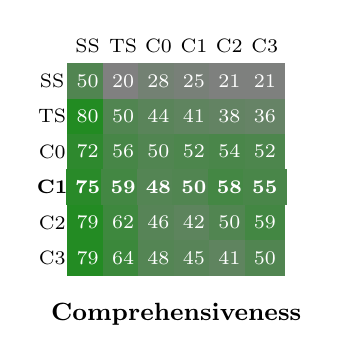
\begin{tikzpicture}[scale=0.45]
  \def\rowlabels{{"SS","TS","C0","C1","C2","C3"}}
  \def\collabels{{"SS","TS","C0","C1","C2","C3"}}
  \foreach \y [count=\n] in {
      {50, 20, 28, 25, 21, 21},
      {80, 50, 44, 41, 38, 36},
      {72, 56, 50, 52, 54, 52},
      {75, 59, 48, 50, 58, 55},
      {79, 62, 46, 42, 50, 59},
      {79, 64, 48, 45, 41, 50},
    } {

      % heatmap tiles
      \foreach \x [count=\m] in \y {
      \pgfmathsetmacro{\z}{(\x-20)*(100/60)}
        \ifnum\n=4
            \node[fill=ForestGreen!\z!gray, minimum size=4.5mm, text=white, font=\scriptsize] at (\m,-\n) {\textbf{\x}};
        \else
            \node[fill=ForestGreen!\z!gray, minimum size=4.5mm, text=white, font=\scriptsize] at (\m,-\n) {\x};
        \fi
      }
    }

  % row labels
  \foreach \a [count=\i] in {0,...,5} {
    \ifnum\a=3
        \node[minimum size=4.5mm, font=\scriptsize] at (0,-\i) {\textbf{\pgfmathparse{\rowlabels[\a]}\pgfmathresult}};
    \else
        \node[minimum size=4.5mm, font=\scriptsize] at (0,-\i) {\pgfmathparse{\rowlabels[\a]}\pgfmathresult};
    \fi
    }
  % column labels
  \foreach \a [count=\i] in {0,...,5} {
    \node[minimum size=4.5mm, font=\scriptsize] at (\i,0) {\pgfmathparse{\collabels[\a]}\pgfmathresult};
  }
  \node[below, align=center, font=\small] at (3.5, -7) {\textbf{Comprehensiveness}};
\end{tikzpicture}
\end{minipage}%
\begin{minipage}{0.25\textwidth}
\vspace*{2mm}
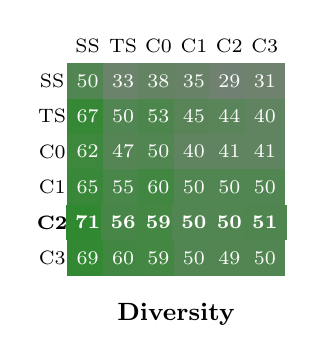
\begin{tikzpicture}[scale=0.45]
  \def\rowlabels{{"SS","TS","C0","C1","C2","C3"}}
  \def\collabels{{"SS","TS","C0","C1","C2","C3"}}
  \foreach \y [count=\n] in {
      {50, 33, 38, 35, 29, 31},
      {67, 50, 53, 45, 44, 40},
      {62, 47, 50, 40, 41, 41},
      {65, 55, 60, 50, 50,50},
      {71, 56, 59, 50, 50, 51},
      {69, 60, 59, 50, 49, 50},
    } {

      % heatmap tiles
      \foreach \x [count=\m] in \y {
      \pgfmathsetmacro{\z}{(\x-20)*(100/60)}
        \ifnum\n=5
            \node[fill=ForestGreen!\z!gray, minimum size=4.5mm, text=white, font=\scriptsize] at (\m,-\n) {\textbf{\x}};
        \else
            \node[fill=ForestGreen!\z!gray, minimum size=4.5mm, text=white, font=\scriptsize] at (\m,-\n) {\x};
        \fi
      }
    }

  % row labels
  \foreach \a [count=\i] in {0,...,5} {
    \ifnum\a=4
        \node[minimum size=4.5mm, font=\scriptsize] at (0,-\i) {\textbf{\pgfmathparse{\rowlabels[\a]}\pgfmathresult}};
    \else
        \node[minimum size=4.5mm, font=\scriptsize] at (0,-\i) {\pgfmathparse{\rowlabels[\a]}\pgfmathresult};
    \fi
    }
  % column labels
  \foreach \a [count=\i] in {0,...,5} {
    \node[minimum size=4.5mm, font=\scriptsize] at (\i,0) {\pgfmathparse{\collabels[\a]}\pgfmathresult};
  }
  \node[below, align=center, font=\small] at (3.5, -7) {\textbf{Diversity}};
\end{tikzpicture}
\end{minipage}%
\begin{minipage}{0.25\textwidth}
\vspace*{2mm}
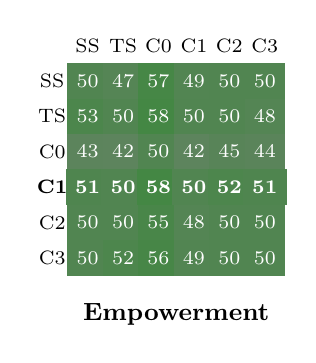
\begin{tikzpicture}[scale=0.45]
  \def\rowlabels{{"SS","TS","C0","C1","C2","C3"}}
  \def\collabels{{"SS","TS","C0","C1","C2","C3"}}
  \foreach \y [count=\n] in {
      {50, 47, 57, 49, 50, 50},
      {53, 50, 58, 50, 50, 48},
      {43, 42, 50, 42, 45, 44},
      {51, 50, 58, 50, 52, 51},
      {50, 50, 55, 48, 50, 50},
      {50, 52, 56, 49, 50, 50},
    } {

      % heatmap tiles
      \foreach \x [count=\m] in \y {
      \pgfmathsetmacro{\z}{(\x-20)*(100/60)}
        \ifnum\n=4
            \node[fill=ForestGreen!\z!gray, minimum size=4.5mm, text=white, font=\scriptsize] at (\m,-\n) {\textbf{\x}};
        \else
            \node[fill=ForestGreen!\z!gray, minimum size=4.5mm, text=white, font=\scriptsize] at (\m,-\n) {\x};
        \fi
      }
    }

  % row labels
  \foreach \a [count=\i] in {0,...,5} {
    \ifnum\a=3
        \node[minimum size=4.5mm, font=\scriptsize] at (0,-\i) {\textbf{\pgfmathparse{\rowlabels[\a]}\pgfmathresult}};
    \else
        \node[minimum size=4.5mm, font=\scriptsize] at (0,-\i) {\pgfmathparse{\rowlabels[\a]}\pgfmathresult};
    \fi
    }
  % column labels
  \foreach \a [count=\i] in {0,...,5} {
    \node[minimum size=4.5mm, font=\scriptsize] at (\i,0) {\pgfmathparse{\collabels[\a]}\pgfmathresult};
  }
  \node[below, align=center, font=\small] at (3.5, -7) {\textbf{Empowerment}};
\end{tikzpicture}
\end{minipage}%
\begin{minipage}{0.25\textwidth}
\vspace*{2mm}
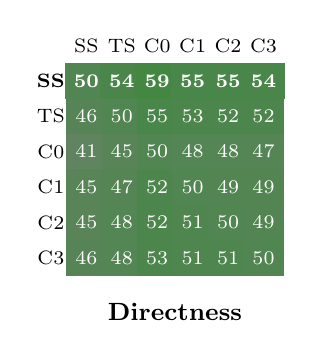
\begin{tikzpicture}[scale=0.45]
  \def\rowlabels{{"SS","TS","C0","C1","C2","C3"}}
  \def\collabels{{"SS","TS","C0","C1","C2","C3"}}
  \foreach \y [count=\n] in {
      {50, 54, 59, 55, 55, 54},
      {46, 50, 55, 53, 52 ,52},
      {41, 45, 50, 48, 48, 47},
      {45, 47, 52, 50, 49, 49},
      {45, 48, 52, 51, 50, 49},
      {46, 48, 53, 51, 51, 50},
    } {

      % heatmap tiles
      \foreach \x [count=\m] in \y {
        \pgfmathsetmacro{\z}{(\x-20)*(100/60)}
        \ifnum\n=1
            \node[fill=ForestGreen!\z!gray, minimum size=4.5mm, text=white, font=\scriptsize] at (\m,-\n) {\textbf{\x}};
        \else
            \node[fill=ForestGreen!\z!gray, minimum size=4.5mm, text=white, font=\scriptsize] at (\m,-\n) {\x};
        \fi
      }
    }

  % row labels
  \foreach \a [count=\i] in {0,...,5} {
    \ifnum\a=0
        \node[minimum size=4.5mm, font=\scriptsize] at (0,-\i) {\textbf{\pgfmathparse{\rowlabels[\a]}\pgfmathresult}};
    \else
        \node[minimum size=4.5mm, font=\scriptsize] at (0,-\i) {\pgfmathparse{\rowlabels[\a]}\pgfmathresult};
    \fi
    }
  % column labels
  \foreach \a [count=\i] in {0,...,5} {
    \node[minimum size=4.5mm, font=\scriptsize] at (\i,0) {\pgfmathparse{\collabels[\a]}\pgfmathresult};
  }
  \node[below, align=center, font=\small] at (3.5, -7) {\textbf{Directness}};
\end{tikzpicture}
\end{minipage}%
\caption{Head-to-head win rate percentages of (row condition) over (column condition) across two datasets, four metrics, and 125 questions per comparison (each repeated five times and averaged). The overall winner per dataset and metric is shown in bold. Self-win rates were not computed but are shown as the expected 50\% for reference. All Graph RAG conditions outperformed na\"ive RAG on comprehensiveness and diversity. Conditions C1-C3 also showed slight improvements in answer comprehensiveness and diversity over TS (global text summarization without a graph index).}
\label{fig:relativemeasures}
\end{figure}